%! Author = Alex
%! Date = 2025-03-18

% Preamble
\documentclass[12pt]{article}
% Formatting imports
\usepackage[
    paper=a4paper,
    top=1in,
    bottom=1in,
    left=1.5in,
    right=1in
]{geometry}
\usepackage{setspace}
% changes the text to double-line spacing
\doublespacing

% Bibliography backend setup
\usepackage[
    backend=biber,
    sortlocale=de_DE,
    natbib=true,
    url=true,
    doi=false,
    eprint=false
]{biblatex}
\addbibresource{refs.bib}



\usepackage[toc,page]{appendix}
\usepackage{amsmath}
\usepackage{caption}
\captionsetup[table]{skip=10pt}

\usepackage{longtable}
\usepackage[table]{xcolor}
\usepackage{tabularx} % Package to manage table width automatically
\usepackage{amssymb}
\usepackage{graphicx}
\usepackage{pdfpages} % Import pdf, used for appendices
\graphicspath{ {figures/} }


% Document
\begin{document}

    % ==================================================
%                    START OF FRONTMATTER
% ==================================================
\pagenumbering{roman}

% Import title page
\begin{titlepage}
    \begin{center}
        
\includegraphics[width=1.0\textwidth]{SCE_banner}
        \vfill
        \vspace*{1cm}

        \Large
        \textbf{Converting Graphical Models}\\
        \textbf{to}\\
        \textbf{Formal Specifications}\\


        \vspace{0.5cm}
        % \LARGE


        \vspace{1.5cm}

        \small
        by\\
        \vspace{0.5cm}
        Alexandre Marques\\
        Student ID: 101189743

        \vfill
        Submitted to: Professor Jason Jaskolka \\
        \vspace{0.8cm}
        Capstone Project - Final Report \\
        SYSC 4907 - Engineering Project

        \vspace{1.5cm}

        % \includegraphics[width=0.4\textwidth]{university}

        Department of Systems and Computer Engineering\\
        Faculty of Engineering\\
        Carleton University\\
        \vspace{1.5cm}
        April 4, 2025

    \end{center}
\end{titlepage}
\addtocounter{page}{1}

% Should we put Acknowledgements?

% Import Abstract section
% ======================================
% How to write an abstract?
% ======================================
% Ref: https://www.anu.edu.au/students/academic-skills/research-writing/journal-article-writing/writing-an-abstract

% Whereas the purpose of an introduction is to broadly introduce your topic and your key message, the purpose of an abstract is to give an overview of your entire project, in particular its findings and contribution to the field. An abstract should be a standalone summary of your paper, which readers can use to decide whether it's relevant to them before they dive in to read the paper.

% Usually an abstract includes the following.
%     A brief introduction to the topic that you're investigating.
%     Explanation of why the topic is important in your field/s.
%     Statement about what the gap is in the research.
%     Your research question/s / aim/s.
%     An indication of your research methods and approach.
%     Your key message.
%     A summary of your key findings.
%     An explanation of why your findings and key message contribute to the field/s.

% It should answer these questions:
% What is your paper about?
% Why is it important?
% How did you do it?
% What did you find?
% Why are your findings important?

% Other version have this simplified structure:
% Background, Methodology, Results, Conclusion

% =================================
% ABSTRACT START
% =================================

\abstract
Formal specifications are a useful method of communicating system descriptions due to their lack of ambiguity,
but they tend to take time to write and require skills few people posses.
In this paper, we propose a way to derive formal specifications from commonly generated informal graphical models.
With our tool, the UML to C2KA Converter (U2C),
we reduce the barriers of formal methods to engineer quality systems.
We managed to read UML State Diagrams to automatically produce Communicating Concurrent Kleene Algebra (C2KA) specifications.
These specifications can be fed to C2KA model checkers, like the Implicit Interactions Analysis Tool (IIAT).
By improving the accessibility of these model checkers, we can identify vulnerabilities and faults earlier in the design process.
This should reduce design cost, and reduce operational damages by helping engineers build safer, and more secure systems.
\\
\textbf{Keywords}: C2KA, UML, Finite State Machine, state diagram, formal methods, model checking, model driven engineering.
% =================================
% ABSTRACT END
% =================================

\newpage

% Automatically generate content lists
\tableofcontents
\newpage
\listoffigures
\listoftables
\newpage


\pagenumbering{arabic}
% ==================================================
%                    END OF FRONTMATTER
% ==================================================

    \section{Introduction}\label{sec:intro}
    \subsection{Problem Background}\label{subsec:problem-background}
Modern system requirements are becoming increasingly complex over time.
To fulfill these requirements, engineers typically go through a modelling phase.
Models are artifacts from the modelling phase which represent different views of the system, in order to understand aspects of the system better.
A common modelling technique is to produce graphical models, in languages such as UML (Unified Modelling Language) to quickly communicate information through visual system interactions.
These visual models are great to communicate understanding across levels of system details between humans,
but they tend to be written with informal modelling languages due to their simplicity.
This means the semantic meaning of the model is nondeterministic, and computers cannot interpret most graphical models.
In contrast, there are formal modelling languages like C2KA (Communicating Concurrent Kleene Algebra) which have a defined semantics.
This allows computers to perform rigorous automated model checking on formal models of the system.
This means critical system properties like safety, and liveness can be proven at the model level before any system implementation starts.

System descriptions can vary in quality, especially across different stages of design.
They can range from informal and incomplete natural language descriptions,
to well-defined formal requirements.
Engineers need to make reasonable decisions on how to model systems from these descriptions.
This often means going for informal visual models which are easy to produce, and communicate with.
Even with their known model checking benefits, formal models are often dismissed.
They require more time to make, but also specialized skills to produce and understand them.
This means formal models cannot easily replace informal models, they typically supplement them.

\subsection{Problem Motivation}\label{subsec:problem-motivation}
We would like to take advantages of the benefits of formal modelling methodologies without having to face the barriers they typically impose.
We believed we could take advantage of the informal models that are typically created to derive formal models with minimal additional cost.
We were specifically interested in the C2KA formalism for a few reasons.
The language is useful for model checking system properties relating to interactions between components, which is an important concern in complex systems with many components.
The language is new, and has low tool support meaning our tool could contribute significantly to its growth.
Experienced C2KA modellers believed this model transformation was possible in this formalism.
This gave us confidence that our project would be feasible, and useful.

% Precise difference between statement, motivation, proposed solution, accomplishments?
\subsection{Problem Statement}\label{subsec:problem-statement}
%This project attempts to reduce the difficulty in creating formal C2KA models by creating them directly from UML State Diagrams.
Our project aims to convert UML State Diagram visual models into C2KA agent specifications.
The goal is to use these agent specifications in our C2KA model checker of interest, the Implicit Interactions Analysis Tool (IIAT).
By targeting a specific model checker, it is easier to prove the function and usefulness of our tool.
We are calling our tool the ``UML to C2KA Converter'', or \textbf{U2C}, for short.

\subsection{Proposed Solution}\label{subsec:proposed-solution}
To achieve this, we decided to find transformation patterns manually first.
Once we understood how to convert it manually, we would encode the rules in a deterministic fashion.
That is, we wanted our program to behave like a pure function.
It should map one given input to exactly one reproducible output.
The output in question would be the agent specification files the IIAT uses.
The input would be some machine-readable version of a set of UML State Diagram.

\subsection{Accomplishments}\label{subsec:accomplishments}
\begin{enumerate}
    \item We found deterministic transformation rules for visual models
    to C2KA specifications.
    \item We managed to read a textual representation of the graphical models.
    \item We re-created a diagram structure to easily parse state diagram information in code.
    \item We used our custom structure to simply implement the transformation rules we determined.
    \item We formatted and serialized our specifications in a format the IIAT could use.
    \item We have created a diff tool to validate our outputs given a trusted C2KA specification written by hand.
    \item We have validated our tool against one known C2KA system, using our diff tool, and by observing parity in the IIAT\@.
\end{enumerate}

\subsection{Document Overview}\label{subsec:document-overview}
The remainder of this report is organized as follows.
Section 2.0 outlines how our project meets the objectives of an engineering project.
Section 3.0 goes over our methodologies and results in technical detail.
Finally, Section 4.0 contains our conclusions, reflexions, and possible future work.

    \newpage

    \section{Engineering Process}\label{sec:eng-process}
    \subsection{Health and Safety}\label{subsec:healthnsafety}

Since we are working on a pure software project,
we do not interact with any dangerous tools or hardware.
The most fearsome tools for us are actually our office peripherals.
We need to be conscious of the ergonomics of our work environment.


% TODO: add ref, https://www.ccohs.ca/oshanswers/ergonomics/office/monitor_positioning.html
Monitor placement is important because it affects eye strain, and postural strain (neck and shoulders).
It is recommended to keep the monitor approximately forty to seventy cm away from the eyes.
For a quick reference, this is roughly an arm's length away, but it depends on the person.
The monitor height is important as well.
In general, research has found that eyes naturally have a downward cast. % REF.
In fact, they strain more looking above, than looking down.
In practice, guidelines recommend keeping the top of the monitor at eye level, or slightly below.
In general, these are just guidelines to get a good starting point.
It may be worth experimenting depending on the individual's body and what feels best.
A visual summary of these recommendations is given by the Canadian Centre for Occupational Health and Safety (CCOHS) in Figure~\ref{fig:monitor-pos}. % TODO Ref here
\begin{figure}[h]
    \centering
    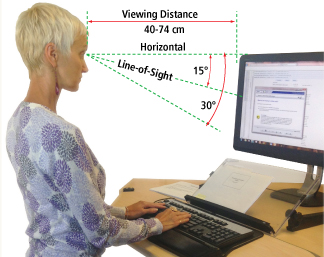
\includegraphics[width=0.5\textwidth]{monitorposition1}
    \caption{The recommended monitor position guidelines from CCOHS.}
    \label{fig:monitor-pos}
\end{figure}

When working for excessively long periods of time without breaks,
it is possible to get repetitive strain injuries (RSI).
It can be from clicking the mouse too much or typing a lot on the keyboard.
Certain mice and keyboards are more ergonomic and help reduce these strains.
They usually have aggressive curves forcing your body to adopt more ergonomic poses.
Office chairs are also an important part of ergonomics, providing proper support while sitting at a desk.

However, even with the best ergonomics setups, the most important is to take frequent breaks from the computer.
Getting up, then walking is good to reduce eye strain, as well as reducing the chances of getting an RSI.
To do this reliably, it is best to set timers and respect them.
Otherwise, there is a risk of getting too absorbed in the work.
After 8 hours of work without breaks writing a report, hands start aching and your body will be the one demanding a break.

% subsection  (end)

\subsection{Engineering Professionalism}\label{subsec:engineering-professionalism}
In ECOR4995, we learned that safety was paramount.

Our first step in addressing this was to analyze the security concerns of our tool.
We do not believe there to be any security vulnerabilities.
This is because it is completely local to the machine, with no internet connection.
We do not believe someone using our tool can harm someone other than themselves by intentionally misusing it.
The only concern would be if an individual delivers falsifies the outputs to provide to someone else.
However, we provide no guarantee for this.
We create text files that can be spoofed without our tool even existing, we decided this concern to be out of scope.

The next question is are there safety concerns, were users can cause harm unintentionally?
We believe there is a way to do so, if our outputs provide false information to a designer.
If the analyzed system is safety critical this can become a safety concern.
The analysis done with our faulty outputs would then compromise the analysis of the safety critical system.
To guard against this, accuracy of our outputs became a critical requirement in our user requirements (see section~\ref{subsubsec:user-reqs}).
We even have a second requirement preferring failure over false positive outputs.

We also made sure to properly licence our program, since we learned that intellectual property was pretty important.

\subsection{Project Management}\label{subsec:project-management}
We started the project by defining some processes for baseline communication and work hours.
That strategy did not work well because we still faced long periods of time without any work or communication.
We had weekly meetings at first, but we wasted time because we had multiple weeks with no work.

The crux of our recovery from this disastrous start came from a pivot towards asynchronous project management with \textbf{GitHub Issues}.
We will look at their purpose in more detail in section~\ref{subsubsec:proj-mngmnt}.
In summary, they were used to formulate task units at a lower level than our requirements.
We could also self-assign the tasks we wanted to do to show to everyone we started work on it.
This is to have a person to contact for status updates, or permission to collaborate on it and avoid duplicating work.

In practice, we stopped doing the assignments because only one person was working for a long period of time.
During the last week before the fair, the team became slightly more active.
Project Management went back to synchronous meetings with dedicated task assignments,
and frequent check-ups to ensure no one was blocked for too long.

We also defined timelines, but they were not respected either.
They only served as a reminder that we were permanently behind schedule, even when we revised our timeline later.
When we switched to Issues, we ended up somewhat ignoring timelines.
We were already working as much as possible until we got blocked, typically due to some lack of understanding of C2KA\@.

Having said that, we still had a clear roadmap of features to follow, and a target date for a first prototype (the fair).
When we were planning tasks, we asked ourselves the feasibility of completion.
This was done in an adhoc manner, based on our knowledge of the current system, and the work left to do.
As we went, we also made sure to mark out of scope features whenever possible (with a rationale) to increase feasibility.

\subsection{Degree Suitability}\label{subsec:deg-suit}

\subsubsection{Alexandre Marques}
This project was suitable to my degree because it touches on many concepts I've learned in class.
It is an engineering project, and it is a software project so it is natural that it fits my Software Engineering degree.
More specifically:
\begin{itemize}
    \item I've applied Project Management techniques from SYSC4106 to increase the chances of completing the project
    \item I've applied Object-Oriented design patterns from SYSC3110 to improve program maintainability and capabilities
    \item I've applied Verification \& Validation concepts from SYSC4101 to increase quality
    \item I've applied CI/CD concepts from SYSC4806 to streamline our development process
    \item I've applied program architecture pattern knowledge from SYSC4120 to select and implement the Pipe and Filter pattern as the best architecture for our goals.
    \item I've applied my knowledge of programming languages from SYSC3101 to select the best language for our needs.
    \item I've applied requirement engineering techniques from SYSC3120 to write a set of functional and non-functional requirements for our program.
    \item I've applied induction rules from COMP2804, COM1805 to implement the recursive logic needed to convert C2KA diagrams (technically learned in SYSC2100 but discrete math taught me recursion much better).
    \item I've applied my Operating System knowledge from SYSC4001 to work on multiple OS hosts and make the IIAT work.
    \item I've applied my knowledge of formal methods from SYSC4111 to identify the importance of formal languages and understand C2KA better.
    \item I've applied my knowledge of modelling from SYSC5805 and SYSC5104 to understand the importance of models in the engineering process.
    \item I've applied my experience in writing technical reports from an academic research internship I've done before the degree,
    combined with the LaTeX skills I've learned during the degree submitting assignments in various classes.
    Although the internship was not part of my degree, it was valuable relevant experience in this domain.
    I was only offered the opportunity because I aimed to do something related to software before even starting the degree.
    \item I've omitted some pre-requisite classes which were not directly relevant,
    but they also contributed to giving me the capabilities to complete this project.
    \item I don't remember when we learned UML and state diagrams.
    It feels like we see them all the time in different classes.
    That was important pre-requisite knowledge too.
\end{itemize}


\subsubsection{Michael Rochefort}

This capstone project integrates and applies a broad range of skills and knowledge from the Software Engineering degree, demonstrating its suitability as a culminating project for the program. At its core, the project required engineering a complex software system from conception to verification, which aligns perfectly with Software Engineering principles. We began with requirements analysis (identifying what the tool needs to do and under what constraints), a process learned in our Requirements Engineering courses. We then moved to software design, selecting an architecture (pipe-and-filter) and design patterns appropriate for the problem. This reflects knowledge from software architecture and design courses, where evaluating and applying architectural styles is a key learning outcome. The implementation involved writing a substantial amount of code in an organized manner, applying best practices for coding and documentation that we developed throughout my degree. Notably, the project’s focus on converting UML models to formal specifications bridged theory and practice: we utilized UML modelling techniques taught in modelling and software design classes, and we engaged with formal methods by generating specifications.

The project also demanded proficient use of software engineering tools and practices. For instance, we used version control (Git/GitHub) extensively – a skill emphasized in our software engineering labs – to collaborate and manage our codebase. We practiced issue tracking and agile-like iteration, echoing project management coursework, to keep the team organized and responsive to changes. The testing strategy we used is a direct application of software testing principles learned in class; we wrote unit tests, integration tests, and system tests much as we would in an industrial setting, reinforcing our understanding of testing frameworks and the importance of test coverage.

Lastly, this project involved teamwork and communication, soft skills that are integral to the Software Engineering program. We had to collaborate effectively, divide tasks, conduct code reviews, and integrate our work, which mirrors the team projects and assignments throughout my degree. The production of a comprehensive technical report and documentation tested my technical communication skills, another key component of the program’s outcomes.


\subsubsection{Ahmed Babar}
The Goal of this project is to streamline and reduce error by creating an automated input for an existing error analysis tool. This project is suitable for the software development degree program as it demonstrates Object oriented programming picked up from courses like 3303 and 2006 where multithreading is used to improve efficiency and 2006 where coupling and techniques were used to create object oriented project just like this one. Another example of use of knowledge from previous course related to this degree include 4001 software validation and 4120 and 3120.

    \newpage

    \section{Technical Details}\label{sec:technical-details}
        \subsection{Background \& Terminology}\label{subsec:background-&-terminology}

\subsection{System Development}
\label{subsec:system-development}
% Change to User requirements?
\subsubsection{User Requirements}\label{subsubsec:user-reqs}

These User Requirements represent our original set of requirements, with minimal implementation details, and domain knowledge.
They are elicited from initial discussions with our supervisor,
and interpretations of the problem statement.
We did not establish a procedure for explicit lower level requirements after this stage.

Some limitations of this process is a lack of explicit detail, priorities, or levels of satisfaction for non-functional requirements.
Instead, we will use later stages of the system development to trace design decisions taken for these requirements.
We will also touch on priorities and possible improvements when we explain
which requirements were skipped for our current release in section~\ref{subsubsec:unsat-reqs}.

The table of requirements contains a list of User Requirements for our system,
with green states indicating satisfactory completion, and gray indicating unsatisfactory:
% Requirement table
\begin{longtable}{|l|p{2.6cm}|l|p{4.5cm}|c|}
    \caption{Set of User Requirements for U2C}
    \label{tab:user-reqs}
    \hline
    \textbf{ID} & \textbf{Requirement} & \textbf{Type}  & \textbf{Description} & \textbf{State} \\
    \hline
    \endhead
    \hline
    % Requirements here
    1 & Input & Functional & U2C shall accept visual system models as input. & \cellcolor{green!30}  \\
    \hline
    2 & C2KA Specifications & Functional & U2C shall interpret given inputs to derive a complete C2KA agent specification. & \cellcolor{green!30}  \\
    \hline
    3 & IIAT Parameters & Functional & U2C shall interpret given inputs to derive the other required IIAT inputs. & \cellcolor{gray!30}  \\
    \hline
    4 & Output & Functional & U2C shall output its computed inputs as text files. & \cellcolor{green!30}  \\
    \hline
    5 & Minimal User Actions & Usability & U2C shall require no additional inputs from the user apart from those required to provide system models. & \cellcolor{green!30}  \\
    \hline
    6 & Modelling Tool Support & Compatibility & U2C shall support models produced by at least one chosen modelling tool (Papyrus, LucidChart, StarUML). & \cellcolor{green!30}  \\
    \hline
    7 & Modelling Language Support & Compatibility & U2C shall support visual models drawn in at least one type of modelling language (ex: UML, SysML, BPMN). & \cellcolor{green!30}  \\
    \hline
    8 & Diagram Type Support & Compatibility & U2C shall support diagrams corresponding to at least one chosen type (ex: state, collaboration, etc.). & \cellcolor{green!30}  \\
    \hline
    9 & Cross Tool Integration & Compatibility & U2C should provide options to integrate directly into tools it depends on (input producer, and output consumers). & \cellcolor{gray!30}  \\
    \hline
    10 & OS Support & Portability & U2C shall run on at least one chosen OS distribution. & \cellcolor{green!30}  \\
    \hline
    11 & Simple System Analysis Speed & Performance & U2C shall produce outputs for a simple system within one minute of execution on a chosen platform specification.
    A simple system is defined as having up to five agents, twenty stimuli, and five behaviours per agent. & \cellcolor{gray!30}  \\
    \hline
    12 & Worst Case Mitigation & Scalability & U2C should scale at a smaller rate than O($n^3$). The expected scaling factors are agents, stimuli, and agent behaviours. & \cellcolor{gray!30}  \\
    \hline
    13 & User Documentation & Maintainability & The U2C code repository shall contain a user manual detailing expected user interactions, and input formats. & \cellcolor{gray!30}  \\
    \hline
    14 & Maintainer Documentation & Maintainability & The U2C code repository shall contain documentation detailing implementation details for maintainers. & \cellcolor{green!30}  \\
    \hline
    15 & Verification Testing & Maintainability & The U2C code repository shall contain automated regression tests providing adequate coverage of the program source code. & \cellcolor{green!30}  \\
    \hline
    16 & Accurate Outputs & Reliability & U2C shall provide deterministic outputs representing accurately what the inputs contain. & \cellcolor{green!30}  \\
    \hline
    17 & No False Positives & Reliability & U2C shall not provide outputs if it cannot find a deterministic interpretation of the given inputs. & \cellcolor{green!30}  \\
    \hline
\end{longtable}

\subsubsection{Chosen Input Type}
The first decision to take concerning inputs was the specific diagram type to support.
This decision impacts the language, since the diagram type may be specific to one or a small set of languages.
It also impacts the modelling tool because it needs to support creating that diagram type.
Most importantly, if the diagram does not have the information we require, there is no purpose in processing it.

Recall that the information we require is related to creating C2KA agent specifications.
Our initial diagram choice was \textit{collaboration diagrams}, due to their simplicity.
When we learned more about C2KA, we realized they do not model agent behaviour very well.
Collaboration diagrams are more suited to describe a specific scenario on an entire system.
Instead, we found that having one \textbf{UML State Diagram} per agent is enough to simply capture agent specifications.
More details on this later when we break down relevant components of state diagrams in section~\ref{subsubsec:input-specification}.

By choosing UML State Diagrams, we also choose \textbf{UML} as our modelling language.
SysML could have been a close viable alternative, but we decided to choose a language we were more familiar with.
This makes it easier to implement properly for us,
but it is also related to our problem statement aiming to use modelling languages already familiar to system designers to reduce the learning curve.
Admittedly outside of software system design SysML is more prevalent, and it is feasible to support both, but we had to limit our scope.

For our modelling tool, we chose \textbf{Papyrus}.
We established evaluation criteria to evaluate different tools, and compared the most popular ones we found.
The most important requirement was machine readability.
We needed to be able to export some representation of the diagram our system could read outside the modelling tool.
Additionally, it was an advantage if it was free, popular, and had ongoing support.
We did not want the modelling tool we depended on to become a hurdle to adopt our program,
ideally we chose a tool which was already in use.
Other tools we looked at were Lucidchart, draw.io, Creately, Gliffy, UMLLet, PlantUML (all had poor export functions),
Modelio (felt hard to use), Astah UML (unpopular),
StarUML and Visual Paradigm (seemed like good alternatives, but we figured out how to use Papyrus first).

To export diagrams from Papyrus, there is an option to export \textbf{XMI files}.
They technically have a .uml file extension in papyrus, but they function the same as XMI files from other tools.
Once a diagram for an agent is finished in papyrus, we can add its XMI file to our program's \textbf{input folder}.
Once all agents are done, we can execute the program.
The user does not need to provide additional inputs.
A full workflow using our program is described in section~\ref{subsec:usage}.

The table below is a traceability summary mapping our original user requirements to the concepts refining them.
Refinements can be correlated by the bolded terms above.

\begin{table}[htbp]
\centering
\caption{Input Decision Requirement Traceability}\label{tab:input-table}
\begin{tabularx}{\textwidth}{| l | l | X |}
    \hline
    \textbf{ID} & \textbf{User Requirement} & \textbf{Refinement} \\
    \hline
    1 & Input & Visual Diagrams are given to the system through XMI file exports from supported modelling tool(s). \\ \hline
    5 & Minimal User Actions & The user puts files in an input folder, then executes the program.  \\ \hline
    6 & Modelling Tool Support & The chosen modelling tool is Papyrus. \\ \hline
    7 & Modelling Language Support & The chosen modelling language is UML. \\ \hline
    8 & Diagram Type Support & The chosen input diagram type is UML State Diagrams. \\ \hline
\end{tabularx}
\end{table}

\newpage
\subsubsection{Input Specifications}\label{subsubsec:input-specification}
Although we accept UML State diagrams, there are specific elements that our interpreter cares about.
The primary goal was to make use of essential model elements only, specifically states and transitions,
to avoid extra modelling requirements.
Unfortunately, modelling expressiveness was a smaller priority, as such
other elements may cause unexpected behaviour.
Ideally, they are ignored.
The next best case is a descriptive error gets raised and crashes the program preventing a faulty output.
In the worst case, an inaccurate specification may be generated without warning.

For the safest behaviour, we have defined a known set of valid model elements, along with usage guidelines.
At a high level, it can be summarized with the class diagram in figure~\ref{fig:supportedElems}.
\begin{figure}[h]
          \centering
          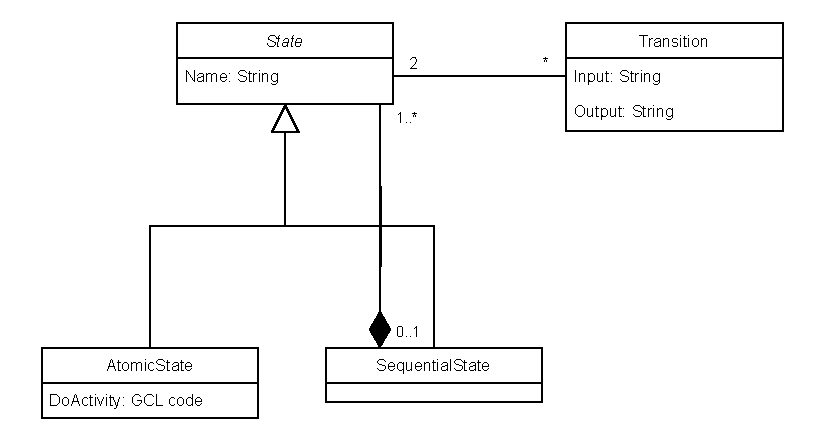
\includegraphics[width=0.5\textwidth]{supportedStateElems.drawio}
          \caption{The class diagram representation of supported diagram elements}
          \label{fig:supportedElems}
\end{figure}
\\
The first element in our state diagram is a \textbf{state}.
States describe a discrete behaviour where an invariant condition holds.
They map directly to \textit{Abstract behaviours} in C2KA\@.
\textbf{Atomic States} are states which do not contain other states.
We can see an example atomic behaviour in figure~\ref{fig:atomicbehaviour}.

\begin{figure}[h]
    \centering
    \includegraphics[width=0.5\textwidth]{Atomicbehaviour}
    \caption{A generic atomic behaviour representation}
    \label{fig:atomicbehaviour}
\end{figure}

Atomic States always have a \textbf{doActivity} property,
as they are needed for C2KA \textit{Concrete behaviours}.
doActivities need to follow Dijkstra's Guarded Command Language (GCL) notation (see ??). % TODO: ref or appendix? what to ref
They are used to assign environmental shared variable values,
with the option to use conditional flows based on the current environment state.
Due to typesetting constraints, we had to convert the GCL operands listed in table~\ref{tab:gcl-equivalence}.
\begin{table}[htbp]
      \centering
      \caption{GCL Conversions for Modelling Tools}\label{tab:gcl-equivalence}
      \begin{tabular}{| l | l |}
          % Header
          \hline
          \textbf{Original GCL} & \textbf{Modelling Tool} \\
          % Header end
          \hline
          $\land$ & \&\& \\ \hline
          $\square$ & $|$ \\ \hline
          $\lor$ & $||$ \\ \hline
          $\rightarrow$ & $->$ \\ \hline
      \end{tabular}
\end{table}
\\

\textbf{Transitions} are links between states which describe how changes in state occur.
We use these transitions and their associated behaviours to compute \textit{Next behaviour} and \textit{Next Stimulus} functions.
For C2KA, we have defined a precise labelling format to follow \{input-stimulus\}/\{output-stimulus\}.
This follows state diagram convention, but it does not allow for guards,
and enforces input and output on all transitions.
\textit{sequential transitions} are special transitions with a single stimulus, their labelling format is: \{in-and-out-stimulus\}.
This is because sequential states use the output of one state as the input of the next state in the sequence.
This allows us to uniquely identify sequential compositions by using a single stimulus as the key identifying property.
We can see an example of transitions and how we interpret mappings from them in figure~\ref{fig:transition}.

\begin{figure}[h]
    \centering
    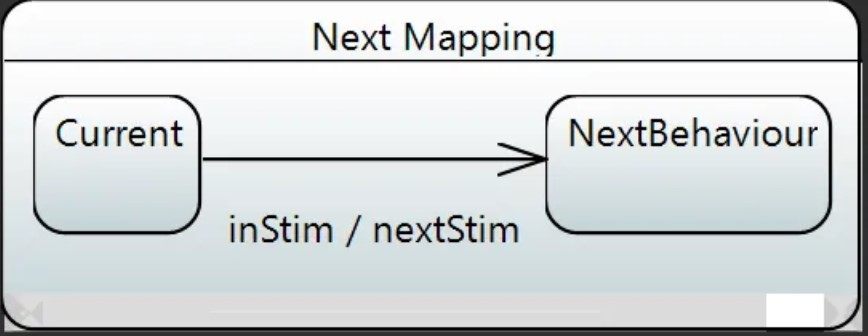
\includegraphics[width=0.5\textwidth]{transitions}
    \caption{A representation of next mappings and their relation to transtions}
    \label{fig:transition}
\end{figure}

\textbf{Sequential States} are super states (state compositions) with a specific composition pattern.
There are at least two inner states.
All inner states are linked by \textit{sequential transitions}.
The sequence has no cycles.
There is a clear initial state with no incoming transitions.
There is a clear final state with no outgoing transitions.
We can see an example sequential state in figure~\ref{fig:sequential}.

\begin{figure}[h]
    \centering
    \includegraphics[width=0.5\textwidth]{Sequentialbehaviour}
    \caption{A C2KA sequential composition represented in a state diagram}
    \label{fig:sequential}
\end{figure}

Note: We explicitly decided not to cover C2KA \textit{parallel compositions} to simplify modelling and parsing.
Instead, a modeller should consider making two different agents which communicate
with each other to model parallel behaviour.

\subsubsection{XMI Parsing}\label{subsubsec:parsing}
% TODO: look at overlap between this and technical background
Having chosen our input format, we needed to find a way to parse it to be able to process it.
Although XMI is supposed to be a standardized format,
many modelling tools will have slight differences for specific components.
Therefore, creating a parser which can be extended generally to support many tools can be challenging.

Thankfully, this is a general problem others have attempted to solve before, and third-party free libraries exist.
We searched for libraries which supported the most recent UML standards, and we were able to make work.
The libraries we tested were \textit{SDMetrics OpenCore},
\textit{eclipse UML2}, \textit{Apache Xerces}, \textit{XMIParser, by cqframework}, \textit{xmiparser, python}.
We only managed to get the \textbf{SDMetrics} Java library to work within our research period.
Since it adequately met our needs, we did not extend the research period to find other alternatives.

The table below traces user requirements to the parsing choices refining them in this section.
\begin{table}[htbp]
    \centering
    \caption{Parser Requirement Traceability}\label{tab:parse-choice-table}
    \begin{tabularx}{\textwidth}{| l | l | X |}
        % Header
        \hline
        \textbf{ID} & \textbf{User Requirement} & \textbf{Refinement} \\
        % Header end
        \hline
        1 & Input & Use SD Metrics OpenCore library to parse XMI file inputs. \\ \hline
    \end{tabularx}
\end{table}

\newpage
\subsubsection{Target Deployment}
One of our user requirements requires us to target an Operating System.
Just like the choice of modelling tool, we want to avoid the OS target to be a barrier to our tool.
We also want to avoid incurring costs attempting to port our tool across multiple Operating Systems.
\textbf{Java} is a great language which allows us to run the same program on any OS due to the Java Virtual Machine.

We considered \textit{C}, but it is not as simple to make platform independent.
\textit{Python} was also a valid alternative because it is also platform independent.
The deciding factor was the availability of third party libraries.
As mentioned in section~\ref{subsubsec:parsing} The SD Metrics library we use for XMI parsing in our system was implemented in Java.
We were not able to make any alternatives work in Python.
With no particular need for other languages, we decided to keep it simple by only using Java in our program.

The table below traces user requirements to the deployment choices refining them in this section.
\begin{table}[htbp]
    \centering
    \caption{Deployment Requirement Traceability}\label{tab:os-choice-table}
    \begin{tabularx}{\textwidth}{| l | l | X |}
        % Header
        \hline
        \textbf{ID} & \textbf{User Requirement} & \textbf{Refinement} \\
        % Header end
        \hline
        10 & OS Support & Use java for platform independence. \\ \hline
    \end{tabularx}
\end{table}

\newpage
\subsubsection{Architecture Choice}
Choosing how to structure our code depends strongly on our functional requirements,
but quality attributes can play a role as well.
The most relevant quality attributes for the architecture for are scalability and performance.
The other requirements are addressed at different steps of the design process.

To begin with, we can think about what our program does not need, like user interaction during execution.
This already gets rid of the need for user interaction focused patterns like \textit{Model-View-Controller} and its variants.
We also have no need for a server or decentralized processing unless we failed to meet our performance goal on one computer.
We did not expect performance to be an issue big enough to require decentralized processing.
Thus, we can eliminate any server patterns, including \textit{microservice} and \textit{service oriented} architectures.

The initial architecture we chose was the \textit{Layer Pattern}, because it fits quite well with the flow of our program.
We are provided an input, and do a series of unidirectional transformations on it to produce an output at the end.
We believed these transformations made sense as different layers of our program.
Layers could pass their outputs through defined input interfaces of the next layer.
This is great for separation of concerns and maintainability.
It is also a great way to reason about the system allowing us to convert our understanding of C2KA transformation to code easily.

That said, we then realized we were starting to describe a \textbf{Pipe and Filter} architecture.
Instead of layers to transform data, we use filters.
We use pipes as our interface to communicate between them.
We still have great separation of concerns, and the same straightforward reasoning for implementation.
The advantage we gain from this pivot is the ability to increase parallelization of processing compared to the layered architecture.
This allows us to directly improve our \textbf{performance} and \textbf{scalability} by reducing the impact of increased data set sizes.

The table below traces user requirements to the architecture choices refining them in this section.

\begin{table}[htbp]
    \centering
    \caption{Architecture Choice Requirement Traceability}\label{tab:arch-choice-table}
    \begin{tabularx}{\textwidth}{| l | l | X |}
        % Header
        \hline
        \textbf{ID} & \textbf{User Requirement} & \textbf{Refinement} \\
        % Header end
        \hline
        11 & Simple System Analysis Speed & Use parallelization enabled by Pipe and Filter to improve performance. \\ \hline
        12 & Worst Case Mitigation & Use parallelization enabled by Pipe and Filter to reduce scaling costs.  \\ \hline
    \end{tabularx}
\end{table}

\newpage
\subsubsection{Architecture Description}\label{subsubsec:arch-desc}
To describe the concrete implementation of our design,
we will break down the responsibilities of our filters, and the pipes in our system through a visual representation.
In these representations, the filters are the named rounded rectangles.
The directional associations show data flow between filters.
Annotations on the data flows specify what data is contained in the pipe.
We also have forks, which are flows going into a black vertical bar and splitting, showing when data is re-used in parallel.
Joins are the opposite operation, collecting data from independent parallel operations back into one centralized point.
Finally, we have the cloud to indicate a simplification in the diagram.
It explains which details were omitted from the model to make it easier to understand.

The first part of our architecture model focuses on converting our expected input to a StateDiagram internally.
% TODO: Model P1 here
When the program starts execution, it reads all the model files at once from a known input address.
It forks once for each model to process them all in parallel.
The first transformation step is to parse the \textit{XMI file} with our \textbf{XMI Parser}.
The parser uses the SDMetrics library to extract generic UML \textit{ModelElements}.

These elements need to be passed to our \textbf{State Diagram Linker}
to build an internal representation of a \textit{state diagram} for our program.
Specifically, we strongly type model elements according to our internally defined types (states, and transitions).
Super states can be thought of as tree roots, and a state diagram can also be represented as a super state.
This allows us to recursively interpret our diagram just like a tree during the following \textbf{diagram interpretation} stage.

The second part of our model completes the process, going from internal StateDiagram to the desired output.
% TODO Model P2
From our \textit{state diagram}, we can perform different analyses in parallel to find parts of the C2KA specification.
The \textbf{abstract behaviour interpreter} looks at super states to find sequential compositions,
and atomic state names to build a C2KA \textit{abstract behaviour specification}.
States which are not sequentially linked are composed by choice.

The \textbf{concrete behaviour interpreter} simply collects all the atomic behaviours and their doActivities.
The doActivities should already be formatted as the concrete behaviour according to our input specification (section~\ref{subsubsec:input-specification}).
The C2KA \textit{concrete behaviour specification} produced is just a formatted collection of the doActivities of the agent.

The \textbf{next behaviour interpreter} checks transitions to find next behaviour mappings.
A mapping is an initial behaviour, an input stimulus, and the resulting behaviour of the transition.
The \textit{next behaviour specification} is the set of all next behaviour mappings found for that agent.

The \textbf{next stimulus interpreter} is essentially the same as next behaviour,
but instead of the resulting behaviour, we check the output stimulus on the transition.
The \textit{next stimulus specification} is the set of all next stimulus mappings found for that agent.

Once all the interpretation is complete, it gets joined into a complete \textit{C2KA Specification}.
We then need to wait at a barrier for all other models to complete analysis before writing our final \textit{output} to a file.

The reason for the barrier is due to a limitation inherent in C2KA of the next stimulus, and next behaviour functions.
They need to be complete functions,
meaning behaviours in an agent need to have defined neutral mappings for all stimuli in the system.
Neutral mappings being outcomes where nothing changes, a neutral stimulus is sent or the behaviour remains the same.
However, since the view of our system is fragmented across our input set,
we cannot identify all stimuli in the system until we analyze all agent inputs to get a complete view of our system.


The table below traces user requirements to the architecture implementations refining them in this section.
\begin{table}[htbp]
    \centering
    \caption{Architecture Description Requirement Traceability}\label{tab:arch-description-table}
    \begin{tabularx}{\textwidth}{| l | l | X |}
        % Header
        \hline
        \textbf{ID} & \textbf{User Requirement} & \textbf{Refinement} \\
        % Header end
        \hline
        1 & Input & XMI Parser, and State Diagram Linker used to convert input to a diagram format we can interpret. \\ \hline
        2 & C2KA Specifications & Interpreter filters are used to convert a diagram to partial C2KA specifications.
        They are then combined into a full C2KA specification. \\ \hline
        4 & Output & The complete C2KA Specification to output conversion allows us to extract agent text files as output.  \\ \hline
    \end{tabularx}
\end{table}

\newpage
\subsubsection{Project Management}\label{subsubsec:proj-mngmnt}
After user requirements, we described our design choices to cover them.
From design, we needed to create tasks to trace the design to specific code implementation.
To do so, we used \textbf{GitHub Issues} to build a list of upcoming tasks for the project.
In figure~\ref{fig:sampleIssueList}, we show a small sample of these issues completed over the course of the project.
\begin{figure}[h]
    \centering
    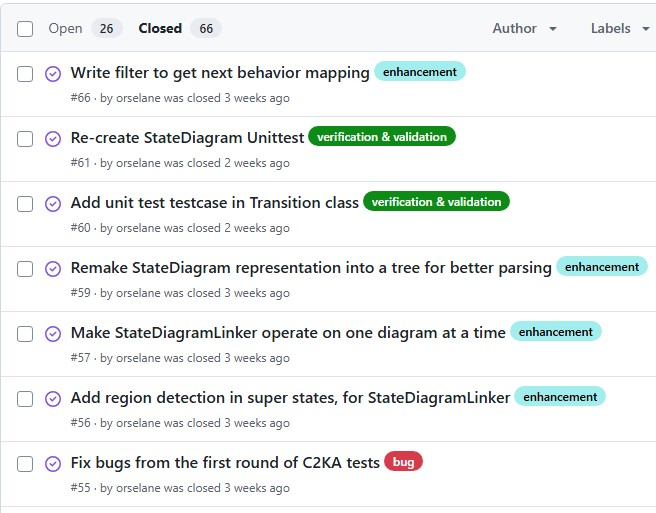
\includegraphics[width=0.8\textwidth]{issueSample}
    \caption{Sample Set of completed issues in our repository}
    \label{fig:sampleIssueList}
\end{figure}

These issues allowed us to assign them when resources were available, and communicate task dependencies easily.
Work done by individuals can be tracked through issues,
preventing multiple people from working on a task simultaneously unaware.
The transition from weekly meetings to asynchronous communication through issues improved our efficiency immensely.
We also customized issue tags to categorize issues
according to our major development concerns, as seen in our repository in figure~\ref{fig:issueTypes}.
\begin{figure}[h]
    \centering
    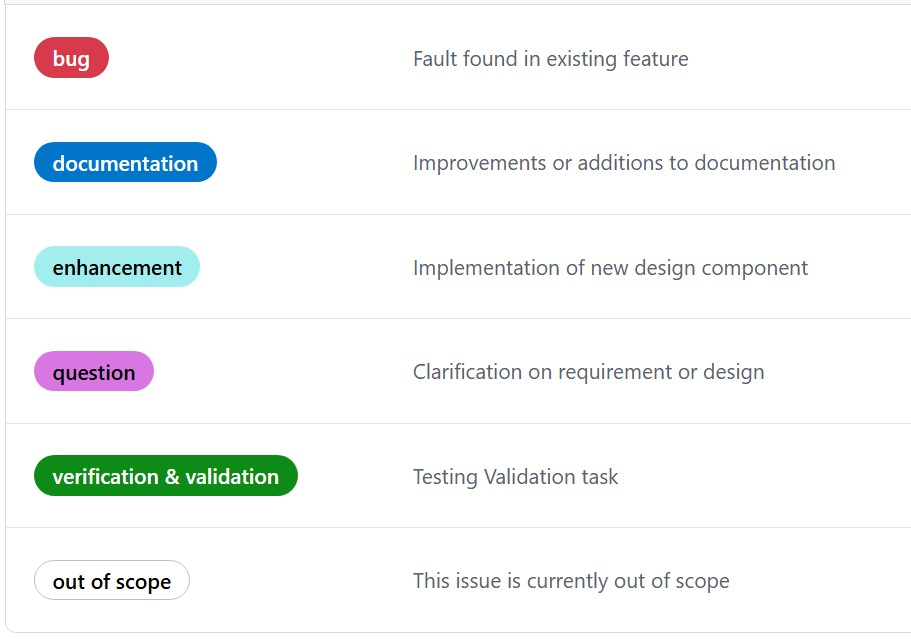
\includegraphics[width=0.8\textwidth]{issueTypes}
    \caption{Types of issues defined in our GitHub repository}
    \label{fig:issueTypes}
\end{figure}

\textit{Enhancements} and \textit{bugs} both relate to implementing our design,
but bugs are errors we found after merging the initial enhancement implementation.
\textit{Verification \& Validation} (V\&V) Tasks related to verifying our code, and validating it.
Usually through creating new tests, but it can also include creating tools for testing,
or establishing and documenting V\&V requirements or strategies.

\textit{Questions} are typically related to clarifications on requirements,
or designs which require research or input from our supervisor.
Once a question is answered, we typically reply directly in the question issue and close it.
Usually, questions have a purpose and can create new issues or unblock existing ones as well.
\textit{Documentation} Tasks related to documenting our project, for any audience.
This includes documentation like this report, function descriptions in code, and a user manual.

\textit{Out of scope} Marks tasks which we identified as out of scope for our current release.
These can include requirements we create to explicitly exclude from the start,
or existing issues we drop later due to time constraints.
In the case where an issue is deemed irrelevant, we do not mark it out of scope.
Instead, we close the issue with a comment for rationale and stop tracking it.
On release, we reset the scope constraints by removing this label on all issues.
After an evaluation of the goals of the next release,
maintainers can decide which issues should stay within the scope of the next release.

We did not develop a great way to automatically trace issues to design,
and we have too many issues to go through them all (over 60 closed issues currently).
Unfortunately, this means we cannot rely on design to code traceability.
Instead, we rely only on testing for validation.
We can, however, demonstrate how we could attempt to manually show traceability through a specific issue.
\begin{figure}[h]
    \centering
    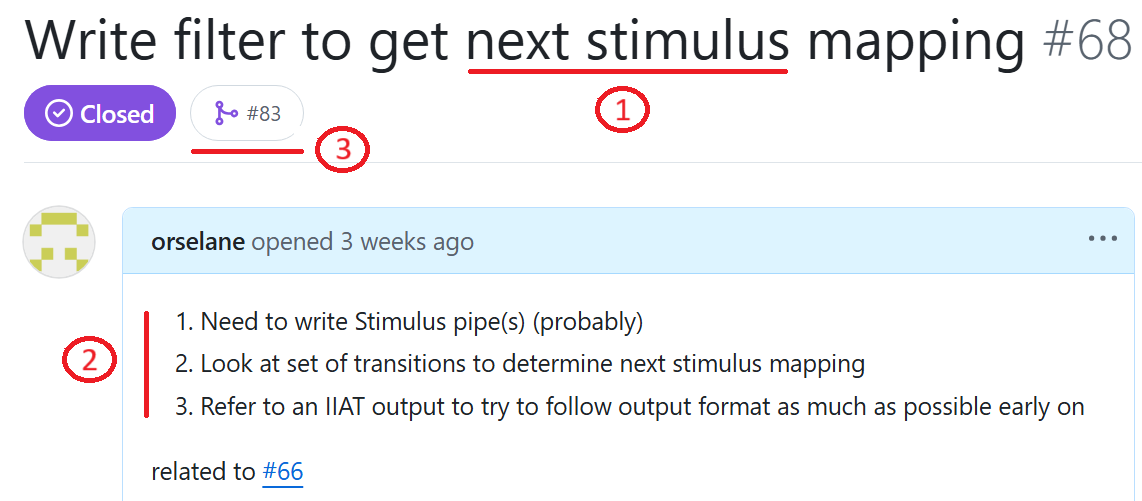
\includegraphics[width=1\textwidth]{specificIssue}
    \caption{An annotated enhancement type issue}
    \label{fig:specificIssue}
\end{figure}
In figure~\ref{fig:specificIssue} we can identify from the title (1) the user requirement the issue contributes to.
In this case, it contributes to the C2KA Specification transformations (User Requirement 2).
Then we can look at the description (2) to see a lower level, but informal explanation to guide the code implementation.
Finally, we see the merged branch (3) linking the issue to merged code changes.

\newpage
\subsubsection{Testing Strategy}\label{subsubsec:tests-strat}
Although we never defined a formal test selection criteria,
we defined informal guidelines to define how to verify our code.

For our simplest code unit, \textit{pipes}, we can \textbf{unit test} it.
After construction, we verify public attributes are as expected.

For \textit{filters}, we did \textbf{integration tests} to more closely simulate a real program environment.
For these tests, we called all the filters up to and including the filter under test then evaluated the output.
This allowed us to do iterative development when we developed new filters,
ensuring new filter implementations were not breaking any previously implemented filters.
The following diagram shows how an integration test would like when testing the State Diagram Linker.
% TODO Make a diagram to show a test on XMI parser

For integration test inputs, we defined a group of elementary C2KA representations which implement
all the elements specified as part of our input specification.
The diagrams used are the same diagrams included in the input specification section~\ref{subsubsec:input-specification}.

For the complete \textit{C2KASpecification} we did end to end \textbf{system tests}, with a \textbf{custom diff tool}.
To do this, we needed a system with known C2KA outputs.
We got analyzed systems from our supervisor, which we treated as the source of truth.
Then, we also needed to model diagrams representing those specifications.
Finally, we create a test with the diagrams as inputs, the analyzed system as expected outputs,
and compare them with our diff tool.

The reason we needed a custom diff tool is due to the inevitable differences between manual C2KA analysis,
and our automated analysis.
There may be some whitespace differences or a different ordering of lines
which are both semantically irrelevant to the specification.
This is why our diff tool checks for an exact match for lines in a specification type,
regardless of their location within the block or any whitespace.
This means that if our actual produced output is missing a line, the diff raises an error,
but it also raises one if our output has an extra line which is not in the expected output.

% TODO show output differences

The table below traces user requirements to our testing strategy concepts refining them in this section.
\begin{table}[htbp]
    \centering
    \caption{Testing Strategy Requirement Traceability}\label{tab:test-strat-table}
    \begin{tabularx}{\textwidth}{| l | l | X |}
        % Header
        \hline
        \textbf{ID} & \textbf{User Requirement} & \textbf{Refinement} \\
        % Header end
        \hline
        15 & Verification Testing & Unit tests, Integration tests provided confidence that our code was continuously functional as we progressed. \\ \hline
        16 & Accurate Outputs & The system tests and diff tool were part of our validation activities to verify output accuracy. \\ \hline
        17 & No False Positives & The system tests should show failures if an output could not be completed, otherwise the diff tool should raise an error. \\ \hline
    \end{tabularx}
\end{table}
\newpage
\subsubsection{Validation Results}\label{subsubsec:test-validation}
% TODO: Complete validation tests before doing this section

The table below traces user requirements to our testing results refining them in this section.
\begin{table}[htbp]
    \centering
    \caption{Validation Requirement Traceability}\label{tab:test-res-table}
    \begin{tabularx}{\textwidth}{| l | l | X |}
        % Header
        \hline
        \textbf{ID} & \textbf{User Requirement} & \textbf{Refinement} \\
        % Header end
        \hline
        1 & Input & Functional part of the end to end testing. \\ \hline
        2 & C2KA Specification & Functional part of the end to end testing.\\ \hline
        4 & Output & Functional part of the end to end testing.\\ \hline
        16 & Accurate Outputs & User . \\ \hline %TODO, fill
        17 & No False Positives & . \\ \hline %TODO, fill
    \end{tabularx}
\end{table}

\newpage
\subsubsection{Unsatisfied Requirements} \label{subsubsec:unsat-reqs}
As we progressed in the project, some lower priority requirements had to be cut to reduce the scope.

For functional requirements, this meant the \textbf{IIAT Parameters}.
Although these are nice to have, they may have required support for an additional diagram type for small benefits.
The core goal of our program was producing the C2KA Specification transformation.

For non-functional requirements, we completely dropped \textbf{cross tool integration}.
It seemed complex, yet not essential to prove one version of our program was functional.
We also cannot claim \textbf{performance} nor \textbf{scalability} of our program due to lack of testing or proofs.
In theory, these properties should hold with our current design, but we did not take the time to prove it.
We did not complete \textbf{User Documentation} adequately, instead focusing on building a comprehensive report.
The user manual should have been the essential sections of the report a user should be aware of,
formatted in a way which makes it easy to learn about and use our project.

We also completed some non-functional requirements but in a way that could be improved.
Our parser allows for multiple \textbf{modelling tool support}, but it still needs to be tested.
Similarly, we could have potentially supported multiple \textbf{modelling languages} with little extra effort.
The same may apply to \textbf{diagram types}.
All of this requires additional tests, and may lead to small tweaks increasing our scope beyond what we could handle.

\textbf{Maintainer documentation} is good, but it is not systematic.
There is no automatic way to detect missing documentation to ensure full functional coverage.
It may also have been good to have a maintainer manual alongside the user manual.
It could explain design decisions and the program architecture at a lower level than the report for overarching context.
For now, this report serves adequately for a system specification.

Our custom diff tool was also not systematically tested.
This means the reports we rely on for accuracy validation may be inaccurate themselves due to an unknown fault in the diff tool.
If we had more time, getting better assurance of our diff tool itself would increase our assurance in the program's overall
\textbf{Reliability}.

In summary, OS Support and the main functions are the only requirements we have fully covered (green).
All other requirements are either adequately covered (also green), or not covered (gray),
as seen in our user requirement table, table~\ref{tab:user-reqs}.


\subsection{Usage}\label{subsec:usage}
\subsubsection{Demonstration Scope}\label{subsubsec:scope}
The demonstration will be using inputs generated to simulate the Manufacturing Cell system seen in section~\ref{subsubsec:c2ka-agents}.
The IIAT tool is pre-configured for this system, and the sample inputs from our V1 release is for this system as well.

To use our tool, we will show the full process from how to generate the inputs,
up to how to provide to our target model checker (IIAT), and the output generated.
We will assume the reader is familiar with the input specification from section~\ref{subsubsec:input-specification},
and how to create their desired state diagram following the specification.
Therefore, we will start by showing how to export an existing state diagram in Papyrus.

Recall that we already deemed the IIAT specific properties out of scope in table section~\ref{subsubsec:unsat-reqs}.
For this version of our program, we do not take responsibility for IIAT configurations to run any Model.
We only wish to demonstrate the C2KA specifications are accurate, and can be used irrespective of the modelling tool.
Showing parity with the existing samples for IIAT is the limit of our demonstration.


% TODO: make sure to name our tool early in the report
\subsubsection{Exporting Inputs from Papyrus}
The first step in providing inputs is to export them from Papyrus.
Figure~\ref{fig:export-1}, Figure~\ref{fig:export-2} and Figure~\ref{fig:export-3} will demonstrate the steps required to do so:
\begin{figure}[h]
    \centering
    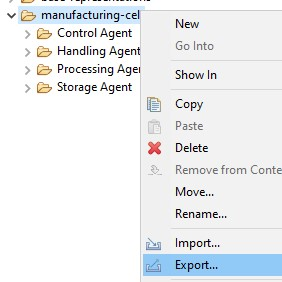
\includegraphics[width=0.5\textwidth]{export-1}
    \caption{Step 1, open export wizard in papyrus]}
    \label{fig:export-1}
\end{figure}
\begin{figure}[h]
    \centering
    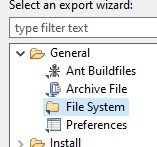
\includegraphics[width=0.5\textwidth]{export-2}
    \caption{Step 2, select file system export}
    \label{fig:export-2}
\end{figure}
\begin{figure}[h]
    \centering
    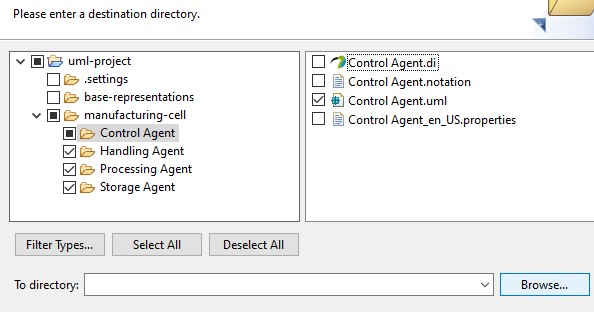
\includegraphics[width=0.5\textwidth]{export-3}
    \caption{Step 3, Select an output directory, and optionally unneeded files.}
    \label{fig:export-3}
\end{figure}

\newpage
\subsubsection{Executing U2C}\label{subsubsec:exec}
To use our program, download the 1.0 zip release from GitHub. % TODO: Repo ref here
Then, extract the zip as is to a folder.
Double-click the jar file to execute it (Java 16+ required).
Open the Output folder, there should be four output files corresponding to the sample input.

If the output does not get generated, the program did not succeed.
This is most likely due to an improper java installation.
Attempt to run the Jar file in the console, for example on Windows the command is:
\begin{verbatim}
    java -jar U2C.jar
\end{verbatim}
This should display some error message which is hopefully helpful enough to troubleshoot.
Otherwise, raise a bug on GitHub with steps to reproduce it.
Optionally, contact an individual currently maintaining the tool for help.

If you had no issues, collect the output for use in later steps of this demonstration.
We will use the sample inputs for reproducibility of the demonstration.
To analyze your own system, you would remove all files in Input, Output then put your own ``.uml'' files in Input.
Then, execute the program, collect the outputs, just as we did with the sample.

\subsubsection{Running the target Model Checker, IIAT}\label{subsubsec:iiat-run}
To build and run the IIAT, follow the instructions on the IIAT repository to install its dependencies first. % TODO: reference to repo here?
We personally recommend avoiding windows, it tends to be more difficult to work with.
The next section assumes you have completed the \textit{Installation} section of the IIAT repository's readme file.

Before running the program, it needs to be compiled locally.
When we tried to do so on our Linux installation, the compiler was having trouble loading \textit{hidden} packages.
These were packages which were installed, but not explicit dependencies of the project.
To fix this issue, we went into the Makefile, and changed the HSFlags variable to add the hidden packages:
\begin{verbatim}HSFlags = -O2 --make -w -package parsec -package vector -package split\end{verbatim}
Admittedly, there must be better fixes, but this was the first time we touched Haskell.
This solution worked well enough to compile and run the program.

Before execution, we also need to configure maude.
Again, we followed the instructions in the source repository.
The only trouble we had this time was finding the file.
It is not specified, but it is located at /src/MaudeInterface.lhs.

For our particular linux installation, we also had to add a missing library.
Specifically, we were missing ``libtinfo.so.5''.
For Arch Linux, we get a ``libtinfo.so.6'' library as a dependency of ncurses (which we already had installed).
It is backwards compatible with the old version, so the solution was to create a symbolic link like so:
\begin{verbatim}sudo link /lib/libtinfo.so.6 /lib/libtinfo.so.5\end{verbatim}

To verify the program works, run the executable with:
\begin{verbatim}./ImplicitsInteractionsAnalysisTool\end{verbatim}
The pre-configured system should be the manufacturing cell.
If it worked, it should display the intended interactions.
Afterward, the IIAT starts computing the implicit interactions and printing them as it goes.
The tool is very verbose, as such we only show the output up to the intended interactions in figure~\ref{fig:iiat-out}.
Note, the figure may look strange, but it is the real output.
We had to copy the output from our shell because we did not have a way to screenshot it in our host.
\begin{figure}[h]
    \centering
    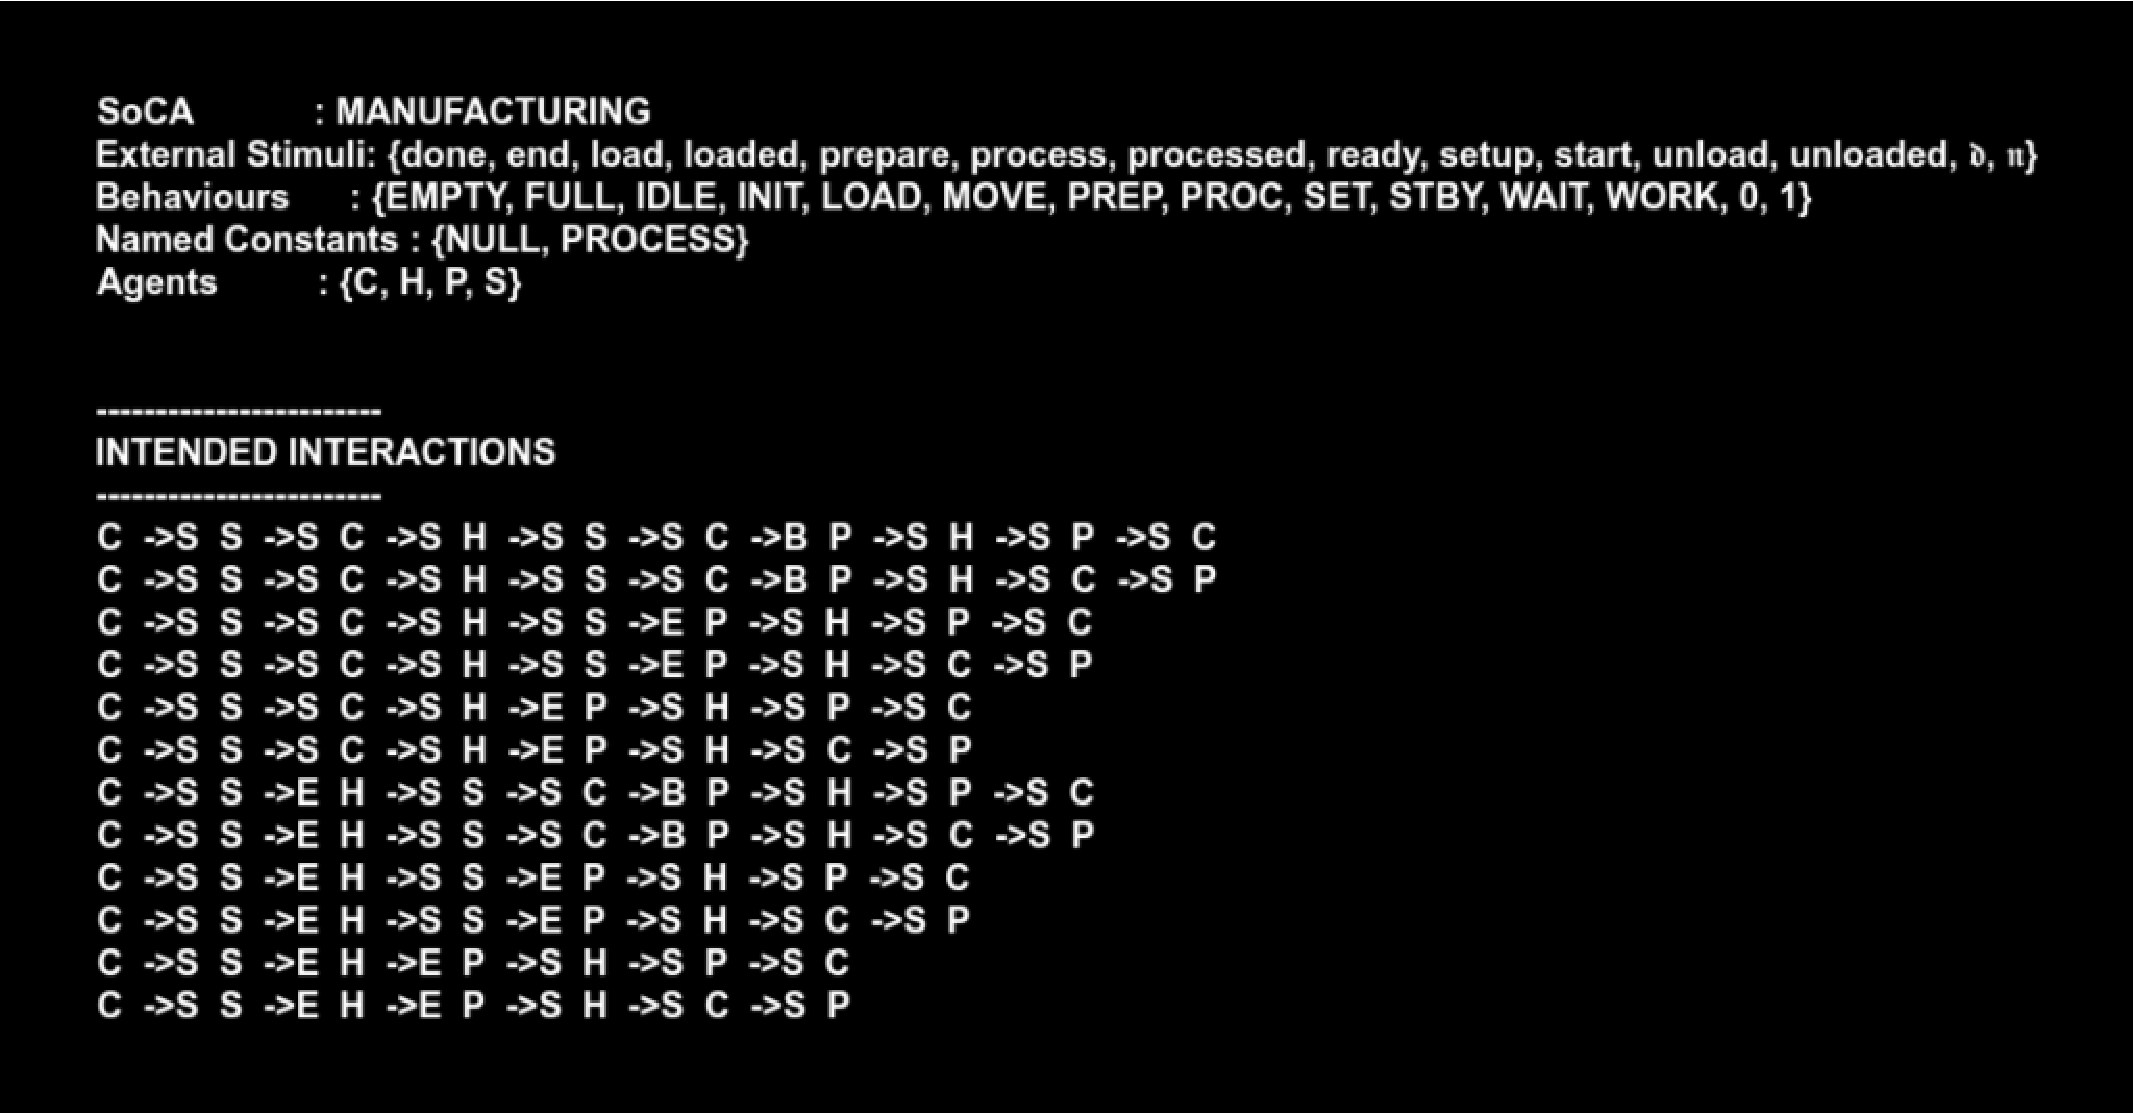
\includegraphics[width=0.6\textwidth]{iiat-out-1}
    \caption{The intended interactions found by the IIAT on the expected input (text copied)}
    \label{fig:iiat-out}
\end{figure}

Note: We did not manage to pipe the output to a file, it has to be observed as it prints currently.
It seems to spawn sub-processes which direct the output to the console directly after the Intended Interactions are printed.
What we did manage to pipe lost its formatting and became difficult to read.
Whichever the case, it seems to be a limitation of the linux implementation.
There may be a way through shell commands to redirect the output, but we are not familiar enough with bash.

\subsubsection{Providing generated specifications to IIAT}
Since the IIAT is pre-configured for the Manufacturing Cell,
we can take advantage of that for this demonstration.
Grab the outputs we generated in section~\ref{subsubsec:exec}.
Replace the files under specs/ManufacturingCell with the outputs generated from our sample input diagrams.
The sample input models the Manufacturing Cell, therefore they should be semantically the same.
You should be able to observe the same outputs from section~\ref{subsubsec:iiat-run} when executing the program again.
Again due to the verbosity, we only check and display the intended interactions in figure~\ref{fig:iiat-out2}.
The output observed was identical from the expected output in figure~\ref{fig:iiat-out}.
\begin{figure}[h]
    \centering
    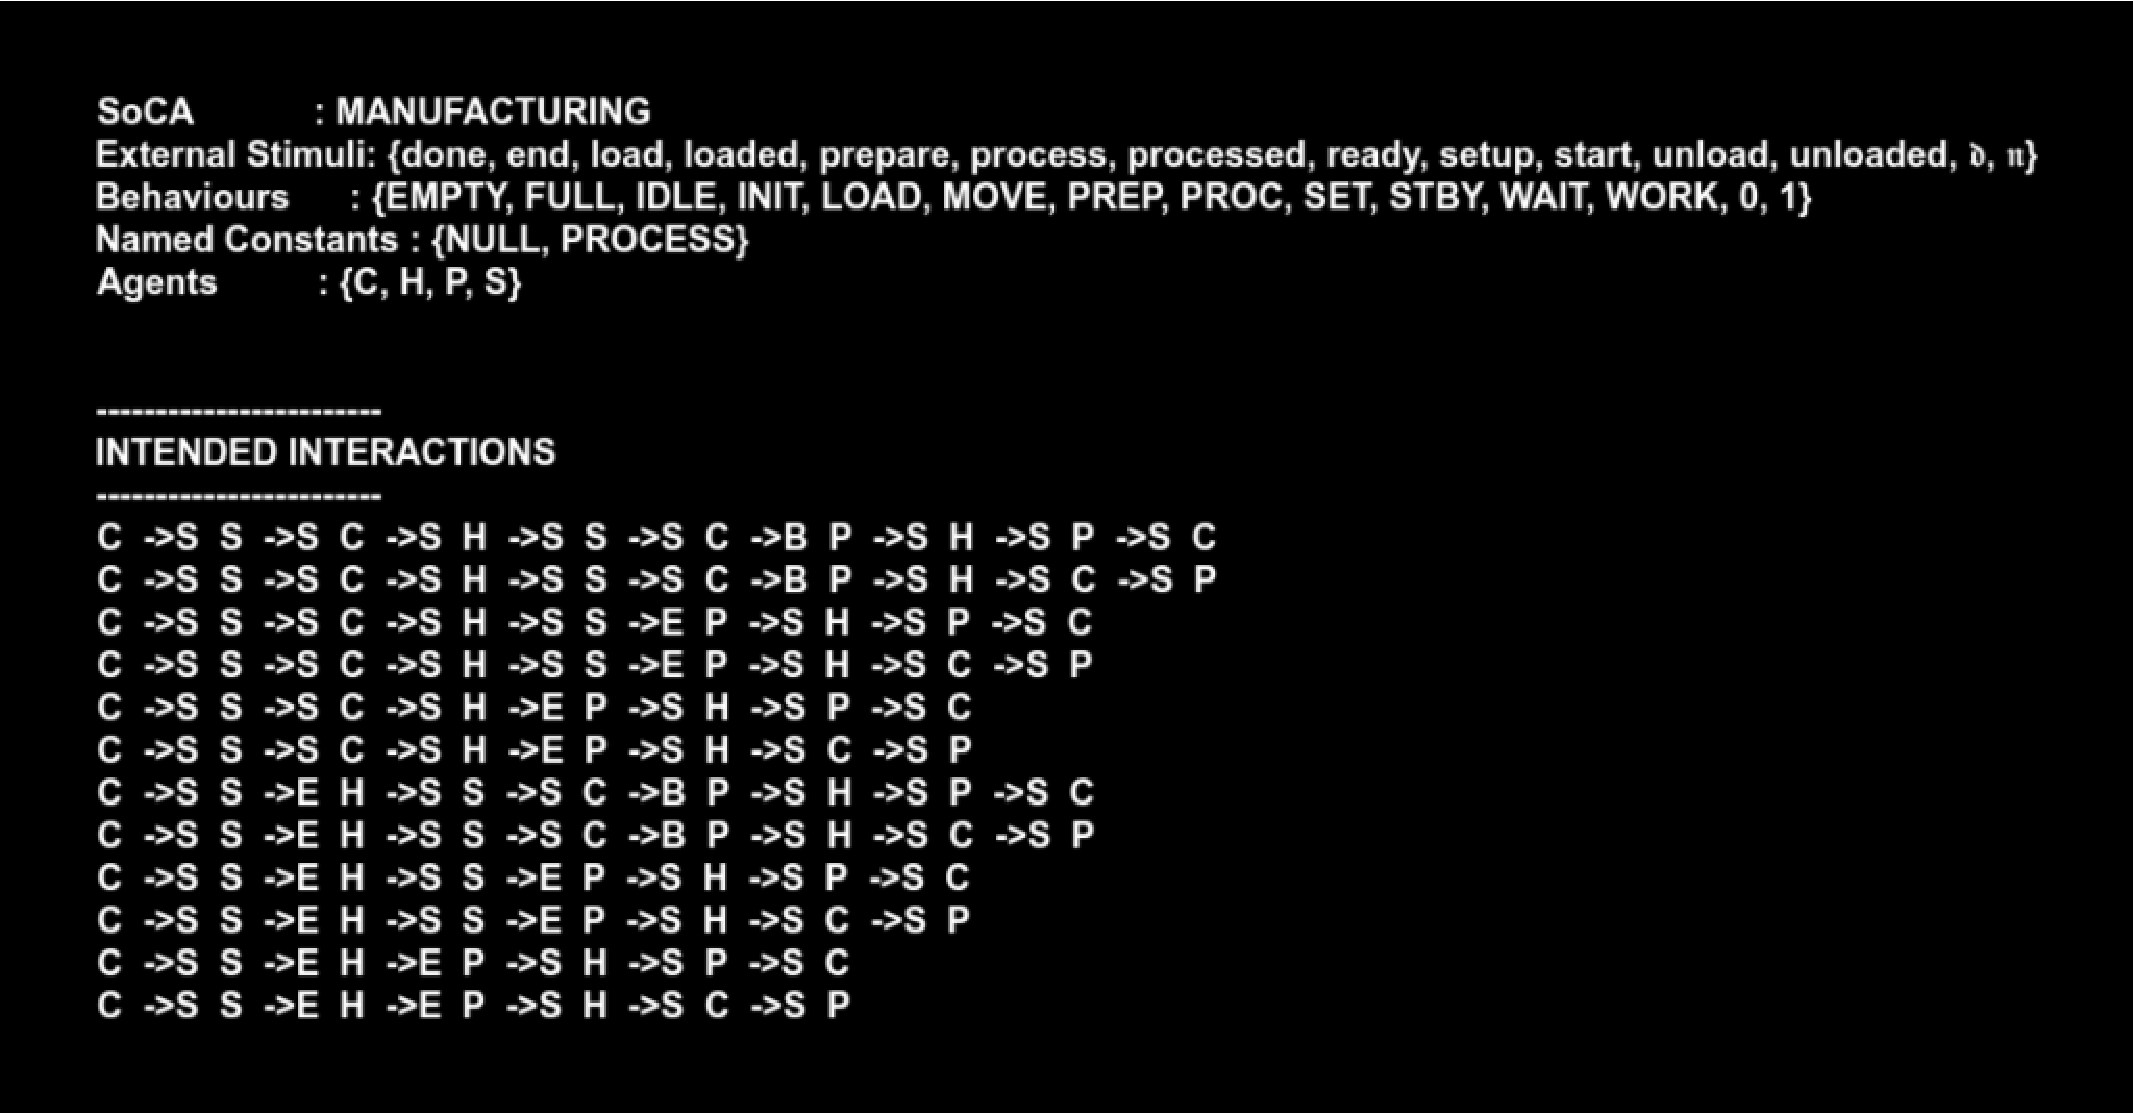
\includegraphics[width=0.6\textwidth]{iiat-out-2}
    \caption{The intended interactions found by the IIAT on our generated specifications (text copied)}
    \label{fig:iiat-out2}
\end{figure}
To analyze different models, additional inputs need to be provided to the IIAT\@.
It does not seem that the IIAT tool explains how to configure the system in the readme.
As such, doing it ourselves for demonstration may require significant exploration.
This is why we deemed it out of scope when we discussed the demonstration scope in section~\ref{subsubsec:scope}.
    \newpage

    \section{Conclusion}\label{sec:conclusion}
    We wanted to find a way to produce C2KA system specifications in an easier way.
C2KA specifications are a useful formalism to analyze systems, but they take time and knowledge to produce.
As such, other methods to gain assurance in a system are used.
These are typically lower in cost, but cannot provide the same degree of assurance (like unit testing code).

We believed that we could leverage a more universal skill than C2KA specification writing:
creating visual diagram representations of the system.
Visual diagrams have the added benefit of being artefacts useful on their own already.
This means users of our tool may already be using them, or benefit from their creation.

The prototype we've built takes in UML state diagrams and can produce C2KA specification files for each agent in the system.
On their own, they can provide a comprehensive overview of the possible behaviors of an agent in the system.
When fed to other analysis tools like the IIAT,
these specifications can also be used to analyze the system for implicit interactions.
These implicit interactions may be the source of hidden vulnerabilities in the system,
which we can now help detect easily.

\subsection{Further Recommendations}\label{subsec:further-recommendations}
There are a few gaps in our prototype compared to our requirements.
For an up-to-date detailed account, our GitHub issues should be the best source in case of any changes after this report was written.
For consistency, we will follow the issue categories we used in GitHub to discuss our recommendations.
See section~\ref{subsubsec:proj-mngmnt} for definitions of these categories.

\subsubsection{Verification \& Validation}\label{subsubsec:rec-v-v}
We are lacking a formal definition of coverage criteria.
The test strategy we defined does a good job at capturing the idea behind how we try to cover tests.
Formalizing coverage criteria would be taking these ideas and formulating them in a way that we can systematically
test our code coverage, and build a report to see if we conform to our desired coverage.
This report would also be an important baseline for assurance in our software.
Checking coverage is done manually at the moment, we make issues if we notice missing coverage (easy to miss).

We also lack system test (validation tests) variety.
It would have been nice to have system tests to test other metrics than ``accuracy'' of our system.
We have no stress tests for performance for example.
This is partially due to a late definition of our non-functional requirements,
as explained later in section~\ref{subsubsec:req-elicit-refl}.

In general, more tests.
We are currently lacking coverage (verification).
More system tests increase assurance in our system (validation), we have very few of them at the moment.

\subsubsection{Enhancements}
The main feature we are lacking is collaboration diagram processing.
We cannot produce an intended sequence of inputs for the IIAT, which was part of our initial set of functional requirements.

Another notable mention was performance improvement related fixes.
Our testing did not yet support proper analysis for these changes, thus work on them did not get started either.

We entertained the idea of having a separate model checker module as part of our tool.
We could have a separate pipeline that could be called independently if desired to check the validity of the inputs.
We would define rules in the module to check the assumptions we defined in section~\ref{subsubsec:input-specification}.
This would help prevent potential unexpected behaviors (false positive outputs),
and it could help improve the error messages we give to users to make fixing user diagrams easier.
The side benefit is by trying to make the artefacts work for our tool,
we may improve diagram quality by automatically reviewing them through our model checker.


\subsubsection{Bugs}
There are none (that we know of!).

In this context, we will count bugs as faults which could lead to an incorrect output being produced.
If the program crashes before producing the output, we may count it as a missing feature depending on the cause.
A well-formed input which crashes means we have not developed the tools to process it yet.
Collaboration diagrams could fall in this category, although we have not yet defined what is a well-formed collaboration diagram either.
Otherwise, it is good if the program crashes because it means that it detected a fault in the input.
If it did not, it would be a bug because the output is faulty (false positive output).

Our philosophy as we were finishing our prototype was to focus on fully functional essential features over many potentially broken features.
The hope is that we may not be able to output everything, but what we do produce can be relied on.


\subsection{Reflections}\label{subsec:reflections}
\subsubsection{Requirement Elicitation Phase}\label{subsubsec:req-elicit-refl}
This section refers to how we collected background information, and determined our requirements from there.
This does not refer to how we managed requirements after we started the implementation.
The issue with this phase is two-fold.
We took way too much time (we did not start implementation work until after the progress report),
and it was not productive given the time spent in it.
Although the User Requirement list in section~\ref{subsubsec:user-reqs} is adequate,
it was never formally defined until the report was written.

At multiple times during implementation, progress halted due to a lack of C2KA knowledge,
or we had to rewrite code from a poor initial understanding.
We also did not put any effort into approving and tracing any requirements other than our functional objectives.
These functional objectives were based on a specific pipeline configuration which we decided to change later,
and thus were too low-level to base our functional requirements on them.
The non-functional objectives of our system became even more implicit, and were subject to change based on
since there was no traceability for them.
This means any decisions regarding trade-offs in the program were decided based off of what felt best at the time,
not an objective metric measured against non-functional requirements.

Our requirement elicitation should have been more targeted, and produced a Software Requirement Specification document
that we verified, and agreed to conform to.
We should have made a process for ongoing requirement elicitation during development.
In the case of a knowledge gap being identified, we would research or ask questions to fill this gap,
then produce requirements and update our SRS accordingly.
This turnaround should not take more than a week to avoid blocking or reverting changes in the implementation.
The initial requirement elicitation phase may warrant a bit more time allocated.
It takes time to develop this process and learn about the problem domain.
It should not have taken us more than a month,
it is better to fail and identify knowledge gaps earlier than be as inefficient as we were.

\subsubsection{Timelines}
There were a few problems with the initial timeline.
The first one was keeping an optional objective and excluding it from our timeline.
Our timeline represented the worst case scenario to still deliver a prototype.
This meant our target of a high-quality project required us to outperform the timeline we proposed.

We also did not include any slack-time in our project, we included it by allocating extra time instead.
This meant components that had six weeks allocated
to them were really supposed to be implemented in potentially a week or two in normal circumstances.
This, and keeping the optional objective implicit made us quite lax in the early stages of the project.

The timeline was also based on two assumptions which did not hold and made it impossible to achieve.
We had agreed as a team to spend a set amount of hours regularly on the project.
This assumption never held throughout the project.
We also based our timeline on a specific scope, architecture and components.
The moment implementation started, we rewrote most of it because we changed our target diagram type.

\subsubsection{Well-Defined Testing Criteria}
As mentioned in our further recommendations in section~\ref{subsubsec:rec-v-v}, our testing could use improvements.
Ideally, after designing our architecture we could have defined test selection and coverage criteria.
If we agreed on it, we could have had an automated mechanism to check our test coverage to see if we're missing tests.
This should have helped us improve our test coverage and build a better case for assurance in our tool.

This would massively improve our verification process.
It would also help with validation because it is much easier to trace well-defined test criteria.
It should also indicate to us early on when we are missing system tests for validation.
In hindsight, we realized quite late what sorts of tests we could make which are not directly linked to the functional output.
These are related to properties like portability, compatibility, and scalability for example.
    \newpage

    \printbibliography
    \newpage

    \begin{appendices}
\section{Project Proposal}\label{ch:project-proposal}\\
\vfill

\includegraphics[width=0.9\textwidth]{appendices/ProposalTitle}
\vfill
\newpage
\includepdf[pages={2-},scale=1]{appendices/4907Proposal.pdf}
\end{appendices}



\end{document}